\chapter{Conclusion}

\section{Results discussion}

The system processes data from the image sensor one pixel column at a time. In each processed pixel column the zero-crossing module will find an index where the zero-crossing happens. This index is the location of the point of maximum intensity on the laser line. Figure \ref{fig:filtered_ex_result_1} shows the result of passing an image through the system. The red line highlights the points of maximum intensity detected by the system.


\begin{figure}[h]
    \centering
    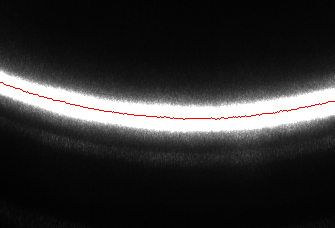
\includegraphics[width=0.4\textwidth]{filtered_ex_result_1.png}
    \caption{Example processing result}
    \label{fig:filtered_ex_result_1}
\end{figure}


The system produces accurate results when the images are not noisy nor highly exposed. The fix for noise was addressed by the use of a smoothing filter. But the high exposure produces high intensity patches in the image as shown in Figure \ref{fig:high_exposure_img_ex_1}. The patches skew the result of the zero-crossing detector as well. This is due to the fact that the patches are of saturated intensity which makes it hard for the smoothing filter to get rid off.


\begin{figure}[h]
    \centering
    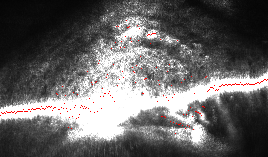
\includegraphics[width=0.5\textwidth]{high_exposure_img_ex_1.png}
    \caption{Skewed results due to over-saturated areas}
    \label{fig:high_exposure_img_ex_1}
\end{figure}


Figure \ref{fig:high_exposure_img_ex_2} shows how the pixel column looks like when the image is exposed for too long. It also shows the detected index is shifted due to the high distortion in the image. A solution to this problem would be to adjust the exposure time according to the material being scanned.


\begin{figure}[h]
    \centering
    \includesvg[width=0.5\textwidth]{high_exposure_img_ex_2.svg}
    \caption{Highly exposed image next to graph of raw and differentiated data}
    \label{fig:high_exposure_img_ex_2}
\end{figure}




\section{Next steps}
\subsection{System optimization}

The design has been implemented in VHDL and its functional behavior has been verified. Afterwards, the design was synthesized for an Intel Cyclone V and achieved a maximum frequency of 228 MHz. However, further speed improvements can be done to increase the clock frequency further. Such as the use of approximated multipliers.

\subsection{Data threshold}

The differentiation filter and the zero-crossing algorithm work better when the noise is eliminated completely from the input pixel data. A method which was tested in the Python script was to cull the data which is below a certain threshold, 80\% of the maximum value is a dataset provided very good results. The issue with this method is that the maximum value is not known beforehand which means that the system needs to read all the values first then calculate 80\% of that value then cull the data points below that value. This introduces large latencies to the system. So, a set threshold or a dynamic threshold could be used on a frame-to-next-frame basis.
